\documentclass[11pt,letterpaper]{article}
\usepackage[utf8]{inputenc} %Codificacion del texto (ISO Latin1 encoding)

\usepackage{fancyhdr} %Permite acomodar a tu gusto la parte de arriba y
% abajo del documento
\usepackage[spanish]{babel} %Permite definir el idioma del dcumento
\usepackage{graphicx} %Permite exportar imagenes en formato eps
\usepackage{url} %Tipo de fuente para correos y paginas
\usepackage{pgf}
\usepackage{fleqn}
\usepackage{amssymb}
\usepackage{fancyvrb}
\usepackage{sectsty}
\usepackage{makeidx}
\usepackage{colortbl} %Permite colocar colores a las tablas
\usepackage{booktabs}
%%%%%%%%%%
%Margenes%
%%%%%%%%%%
\parskip 1mm %Espacio entre parrafos

\setlength{\topmargin}{0pt}

\oddsidemargin	0.5cm  % Ancho Letter 21,59cm
\evensidemargin 0.5cm  % Alto  Letter 27,81cm
\textwidth	15.5cm
\textheight	21.0cm
\headsep	4 mm
\parindent	0.5cm
%%%%%%%%%%%%%%%%%%%%%%
%Estilo del documento%
%%%%%%%%%%%%%%%%%%%%%%
\pagestyle{fancyplain}

%%%%%%%%%%%%%%%%%%%%%%%%%%%%%%%%%%%%%%%%%%%
%Fancyheadings. Top y Bottom del documento%
%%%%%%%%%%%%%%%%%%%%%%%%%%%%%%%%%%%%%%%%%%%
% Recuerde que en este documento la portada del documento no posee
% numeracion, pero de igual manera llamaremos a esa primera pagina la numero
% 1, y la que viene la dos. Esto es para tener una idea de las que
% llamaremos pares e impares
\lhead{Sistemas de Informaci\'on} %Parte superior izquierda
\rhead{\bf \it Tarea 2} %Parte superior derecha
\lfoot{\it M. Porter y los procesos de negocios} %Parte inferior izquierda. \thepage indica
% el numero de pagina
\cfoot{} %Parte inferior central
\rfoot{\bf \thepage} %Parte inferior derecha
\renewcommand{\footrulewidth}{0.4pt} %Linea de separacion inferior

% Challa

\newtheorem{theorem}{Theorem}
\newtheorem{acknowledgement}[theorem]{Acknowledgement}
\newtheorem{algorithm}[theorem]{Algorithm}
\newtheorem{axiom}[theorem]{Axiom}
\newtheorem{case}[theorem]{Case}
\newtheorem{claim}[theorem]{Claim}
\newtheorem{conclusion}[theorem]{Conclusion}
\newtheorem{condition}[theorem]{Condition}
\newtheorem{conjecture}[theorem]{Conjecture}
\newtheorem{corollary}[theorem]{Corollary}
\newtheorem{criterion}[theorem]{Criterion}
\newtheorem{definition}[theorem]{Definition}
\newtheorem{example}[theorem]{Example}
\newtheorem{exercise}[theorem]{Exercise}
\newtheorem{lemma}[theorem]{Lemma}
\newtheorem{notation}[theorem]{Notation}
\newtheorem{problem}[theorem]{Problem}
\newtheorem{proposition}[theorem]{Proposition}
\newtheorem{remark}[theorem]{Remark}
\newtheorem{solution}[theorem]{Solution}
\newtheorem{summary}[theorem]{Summary}
\newenvironment{proof}[1][Proof]{\noindent\textbf{#1.} }{\ \rule{0.5em}{0.5em}}

\newcommand{\primaria}[1]{
	\textbf{\underline{#1}}
}

\newcommand{\foranea}[1]{
	\textbf{\textsl{#1}}
}

\newcommand{\primyfor}[1]{
	\underline{\foranea{#1}}
}

\makeatletter
\newcommand\subsubsubsection{\@startsection {paragraph}{1}{\z@}%
                                   {-3.5ex \@plus -1ex \@minus -.2ex}%
                                   {1.5ex \@plus.2ex}%
                                   {\normalfont\bfseries}}
\newcommand\subsubsubsubsection{\@startsection {subparagraph}{1}{\z@}%
                                   {-3.5ex \@plus -1ex \@minus -.2ex}%
                                   {1.5ex \@plus.2ex}%
                                   {\normalfont\bfseries}}


\makeatother

%\makeindex
%%%%%%%%%%%%%%%%%%%%%%%%%%%%%%%%%%%%%%%%%%%%%%%%%%%%%%%%%%%%%%%%%%%
%%%%%%%%%%%%%%%%%%%% Aqui empieza el documento %%%%%%%%%%%%%%%%%%%%
%%%%%%%%%%%%%%%%%%%%%%%%%%%%%%%%%%%%%%%%%%%%%%%%%%%%%%%%%%%%%%%%%%%

\begin{document}

%%%%%%%%%%%%%%%%%%%%%%%%%%
%Definicion de la portada%
%%%%%%%%%%%%%%%%%%%%%%%%%%
\begin{titlepage}
    \begin{center}
	%\begin{tabular}{ccc}
	\begin{tabular}{c}
		
\includegraphics[width=0.9\textwidth]{img/logos}
		
	   % 
\includegraphics[width=3cm]{img/utfsm}
	   % & 
	   % \hspace{-0.2cm}
	   % \begin{tabular}{c}
	   % Universidad Técnica Federico Santa María \\ \hline
	   % \vspace{0.2cm}
	   % Departamento de Informática\\
	   % \vspace{1.2cm}
	   % \end{tabular}
	   % \hspace{0.2cm}
	   % &
        %    
\includegraphics[width=2cm]{img/di}
	\end{tabular}

	\vspace{4cm}
	%Titulo del Documento
	\begin{tabular}{c}
		\vspace{3cm}
		\Large{\sc{Seminario de Modelos y Métodos Cuantitativos}}\\
		\huge{\sc{Tarea 2}}\\\\
		%\includegraphics[scale=0.7]{img/portada} \\\\
	\end{tabular}

    \vspace{5cm}
	\begin{tabular}{lr}
			\textbf{Alumnos} & \\
							 & \\
         	\normalsize{Cristián Maureira Fredes} & \url{cmaureir@csrg.inf.utfsm.cl}\\
         	\normalsize{Gabriel Zamora Nelson} & \url{gzamora@csrg.inf.utfsm.cl}\\

							 & \\
			\textbf{Profesor} & \\
							 & \\
         	\normalsize{Andrés Moreira} & \url{amoreira@inf.utfsm.cl}\\
	\end{tabular}

\vspace{2cm}

	%Fecha
    \normalsize{\sc{\today}}\\
    %\normalsize \textbf{Fecha de Entrega:} & {14 de Noviembre del 2010}\\
    \end{center}
\end{titlepage}


\section*{\'Indice}
\label{sec:indice}
\vspace{2cm}
\begin{itemize}
	\item Introducci\'on       		\hspace{10cm}    P\'ag. 02\\
	\item S\'intesis del Texto 		\hspace{9.15cm}  P\'ag. 03\\
	\item Rese\~na del Autor   		\hspace{9.19cm}  P\'ag. 05\\
	\item Pensamiento Gestión de Empresas   \hspace{6.35cm}     P\'ag. 06\\
	\item Acerca Procesos de Negocios	\hspace{7.25cm}     P\'ag. 11\\
	\item Conclusi\'on        		\hspace{10.25cm}  P\'ag. 18\\
	\item Referencias          		\hspace{10.25cm} P\'ag. 19\\
	\item Glosario             		\hspace{10.75cm} P\'ag. 20\\
	\item M\'etodo de Trabajo  		\hspace{8.9cm}   P\'ag. 22\\
\end{itemize}
\newpage


\section*{Introducci\'on}
\label{sec:introduccion}
\frame
{
\frametitle{Introducción}
\begin{itemize}
	\item Motivación del problema.
	\item Sobre la técnica.
	\item Implementación inicial.
	\item Sintonización.
	\item \blue{Control}.
	\item Resultados.
\end{itemize}
}



\section*{S\'intesis}
\label{sec:sintesis}
Michael Portes es profesor de Administración de Negocios, en la Escuela de Negocios de Harvard,
y además es una destacada autoridad en Estrategia Competitiva y Competitividad Internacional.

Porter ha escrito más de 16 libros, y también ha publicado más de 60 artículos.

Unas de las ideas principales planteadas por Porter es la de “Cadena de Valor”, ya que puede
orientar a las organizaciones para que redistribuyan sus recursos, con el fin de que mejoren el
rendimiento, y así lograr mejorar la ventaja competitiva. A continuación se hablara algo más de
este tema.

La cadena de valor describe las organizaciones como cadenas causales de actividades, que agregan
valor para los clientes mediante la transformación de insumos en entrega de productos o servicios.

Para el cliente el valor es la suma de los beneficios menos los costos.

Según Porter, al abordarse el diseño estratégico de la organización se configurará en ella una
cadena de valores en forma efectiva, para lo que se debe eliminar las actividades que no agregan
valor a los productos o servicios, y además se tiene que mejorar aquellas que lo agregan. De esta
forma, una organización en la cual se optimizó la cadena de valor está en condiciones de incrementar
sus ventajas competitivas, en materia de costos y calidad, en la medida que pueda satisfacer las
expectativas de los clientes con el mejor precio.

Porter divide las tareas existentes en la empresa en 2 grupos, que son los de actividades primarias
y actividades de apoyo. Las actividades primarias son propias de la empresa, en cambio las de apoyo
generalmente se realizan por empresas externas.

Las actividades primarias son 5, y son las siguientes:
\begin{itemize}
	\item Logística Interna.
	\item Operaciones.
	\item Logística Externa.
	\item Marketing y Ventas.
	\item Servicios.
\end{itemize}
Las actividades de apoyo son 4, y son:
\begin{itemize}
	\item Adquisiciones.
	\item Desarrollo de tecnología.
	\item Manejo de Recursos Humanos.
	\item Infraestructura de la firma.
\end{itemize}
Las actividades primarias debieran ser internas, y se convendría maximizar su rendimiento. En las
actividades de apoyo se debe definir un beneficio mínimo y variar el costo, buscar mejores ofertas en
coste, que cumplan con el beneficio mínimo, o el mejor beneficio a costo mínimo.

Con esto Porter nos dice que toda empresa se puede dividir en 9 actividades, maximizables por distintas
técnicas, para así lograr la mejor oferta para el cliente.

\newpage


%inicio desarrollo

\section*{Rese\~na del Autor}
\label{sec:autor}
\textbf{Michael Porter}\\\\
Nacido en el 1947.Es un académico estadounidense que se centra en temas de economía y administración
de empresas. Actualmente es Profesor en la Escuela de Negocios de Harvard (Harvard
Business School), donde conduce el Instituto para la estrategia y la competitividad
(Institute for Strategy and Competitive).\\

Porter es B.A (Bachellor in Arts) en ingeniería mecánica y aeroespacial, por la
Universidad de Princeton (1969), MBA por la Universidad de Harvard (1971) y Ph.D.
en Economía Empresarial (Business Economics) por la Universidad de Harvard (1973).\\

Su principal teoría es la de Gerencia Estratégica, que estudia como una empresa o
una región pueden construir una ventaja competitiva y sobre ella desarrollar una
estrategia competitiva.\\

En 1984 fue cofundador de Monitor Group, una firma de consultoría en administración
y estrategia.\\

\begin{center}
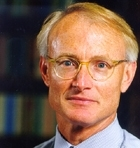
\includegraphics[height=3cm]{images/porter}
\end{center}
\newpage


\section*{Pensamiento de porter en relación a la gestión de empresas}
\label{sec:pensamiento}
\subsection*{El Modelo de las cinco fuerxas de Porter}

El Análisis Porter de las cinco fuerzas es un modelo elaborado por el economista Michael Porter en 1979,
en que se describen las 5 fuerzas que influyen en la estrategia competitiva de una compañía que determinan
las consecuencias de rentabilidad a largo plazo de un mercado, o algún segmento de éste. Las primeras cuatro
fuerzas se combinan con otras variables para crear una quinta fuerza, el nivel de competencia en una industria.

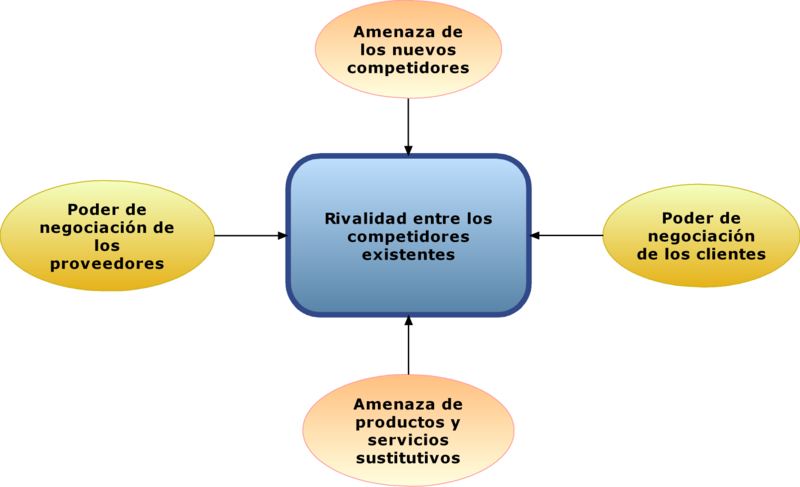
\includegraphics[height=8cm]{images/cincoFuerzas}

\begin{enumerate}
	\item \emph{Entrada Potencial de Nuevos Competidores}
		El mercado o el segmento no son atractivos dependiendo de si las barreras de entrada son fáciles
		o no de franquear por nuevos participantes, que puedan llegar con nuevos recursos y capacidades
		para apoderarse de una porción del mercado.
	\item \emph{Rivalidad entre Empresas Competidoras}
		Para una corporación será más difícil competir en un mercado o en uno de sus segmentos donde los
		competidores estén muy bien posicionados, sean muy numerosos y los costos fijos sean altos, pues
		constantemente estará enfrentada a guerras de precios, campañas publicitarias agresivas, promociones
		y entrada de nuevos productos
	\item \emph{Poder de Negociación de los Proveedores}
		Un mercado o segmento del mercado no será atractivo cuando los proveedores estén muy bien organizados
		gremialmente, tengan fuertes recursos y puedan imponer sus condiciones de precio y tamaño del pedido.
		La situación será aún más complicada si los insumos que suministran son claves para nosotros, no tienen
		sustitutos o son pocos y de alto costo. La situación será aún más crítica si al proveedor le conviene
		estratégicamente integrarse hacia delante.
	\item \emph{Poder de Negociación de los Consumidores}
		Un mercado o segmento no será atractivo cuando los clientes están muy bien organizados, el producto
		tiene varios o muchos sustitutos, el producto no es muy diferenciado o es de bajo costo para el cliente,
		lo que permite que pueda hacer sustituciones por igual o a muy bajo costo. A mayor organización de los
		compradores, mayores serán sus exigencias en materia de reducción de precios, de mayor calidad y servicios
		y por consiguiente la corporación tendrá una disminución en los márgenes de utilidad. La situación se hace
		más crítica si a las organizaciones de compradores les conviene estratégicamente sindicalizarse.
	\item \emph{Desarrollo Potencial de Productos Sustitutos}
		Un mercado o segmento no es atractivo si existen productos sustitutos reales o potenciales. La situación
		se complica si los sustitutos están más avanzados tecnológicamente o pueden entrar a precios más bajos
		reduciendo los márgenes de utilidad de la corporación y de la industria.
\end{enumerate}

\subsection*{Porter y la competitivida}

La competitividad debe ser entendida como la capacidad que tiene una organización, pública o privada, lucrativa o no, de
obtener y mantener ventajas comparativas que le permitan alcanzar, sostener y mejorar una determinada posición en el entorno
socioeconómico. El término competitividad es muy utilizado en los medios empresariales, teniendo incidencia en la forma de
plantear y desarrollar cualquier iniciativa de negocios, lo que provoca, obviamente una evolución en el modelo de empresa y
empresario.

La ventaja comparativa o competitiva de una empresa estaría en su habilidad, recursos, conocimientos y atributos, etc., de los
que dispone, y los mismos de los que carecen sus competidores o tienen en menor medida, haciendo esto posible la obtención de
unos rendimientos superiores a los de aquellos. El concepto de competitividad nos hace pensar en la idea “excelencia”, con
características de eficiencia y eficacia de la organización.

Las empresas competitivas son aquellas capaces de ofrecer continuamente productos y servicios con atributos apreciados por sus
clientes. A este conjunto de características que distinguen al producto de una empresa de sus competidores lo denominamos
ventajas competitivas. Lo único seguro acerca de las ventajas competitivas es su dinamismo; los mercados pueden cambiar sus
exigencias o la tecnología de la empresa puede verse desplazada por las de la competencia. Si una empresa no invierte en
mantenerlas, renovarlas, tarde o temprano estará condenada a perderlas.

Existen dos categorías de ventajas competitivas: de costes y de valor añadido. Las ventajas de costes están asociadas con la
capacidad de ofrecer a los clientes un producto al mínimo coste. Las ventajas competitivas de valor; por su parte, están
basadas en la oferta de un producto o servicio con atributos únicos, discernibles por los clientes, que distinguen a un
competidor de los demás. (Julián Villalba)

Michael Porter afirmaba que la competitividad está determinada por la productividad, definida como el valor del producto
generado por una unidad de trabajo o de capital. Para hablar de competitividad, continúa Porter, habría que irse a la empresa,
y al sector, e identificar cuáles son los factores que determinan que las empresas generen valor añadido y que ese valor se
venda en el mercado, y si realmente esos factores son sostenibles en el mediano y largo plazo.

Asimismo, Michael Porter establece cuatro factores que pueden ser determinantes en la competitividad:
\begin{enumerate}
	\item La dotación del país, en términos de cantidad y calidad de los factores productivos básicos (fuerza de trabajo,
		recursos naturales, capital e infraestructura), así como de las habilidades, conocimientos y tecnologías
		 especializados que determinan su capacidad para generar y asimilar innovaciones.
	\item La naturaleza de la Demanda Interna en relación con la oferta del aparato productivo nacional; en particular,
		es relevante la presencia de demandantes exigentes que presionan a los oferentes con sus demandas de artículos
		innovadores y que se anticipen a sus necesidades.
	\item La existencia de una estructura productiva conformada por empresas de distintos tamaños, pero eficientes en escala
		internacional, relacionadas horizontal y verticalmente, que aliente la competitividad mediante una oferta interna
		especializada de insumos, tecnologías y habilidades para sustentar un proceso de innovación generalizable a lo
		largo de cadenas productivas.
	\item Las condiciones prevalecientes en el país en materia de creación, organización y manejo de las empresas
\end{enumerate}

\subsection*{Arquitectura de la Empresa}

Arquitectura de la Empresa es el conjunto de elementos organizacionales (objetivos estratégicos, departamentos, procesos, tecnología,
personal, etc.) que describen a la empresa y se relacionan entre sí garantizando la alineación desde los niveles más altos (estratégicos)
hasta los más bajos (operativos), con el fin de optimizar la generación de productos y servicios que conforman la propuesta de valor
entregada a los clientes.

De esta definición destaca el hecho de que se busca una alineación de los niveles más altos con los más bajos de la empresa. Esto es
importante, debido a que todas las áreas de la empresa deben actuar en armonía para conseguir los objetivos definidos por la misma.
Esto suena muy obvio, pero en la práctica es frecuente perder este enfoque. La Arquitectura de la Empresa ayuda a conservar la
perspectiva y a garantizar esta alineación. Los diferentes niveles que se tienen que modelar en la arquitectura se explican a continuación:

\begin{center}
	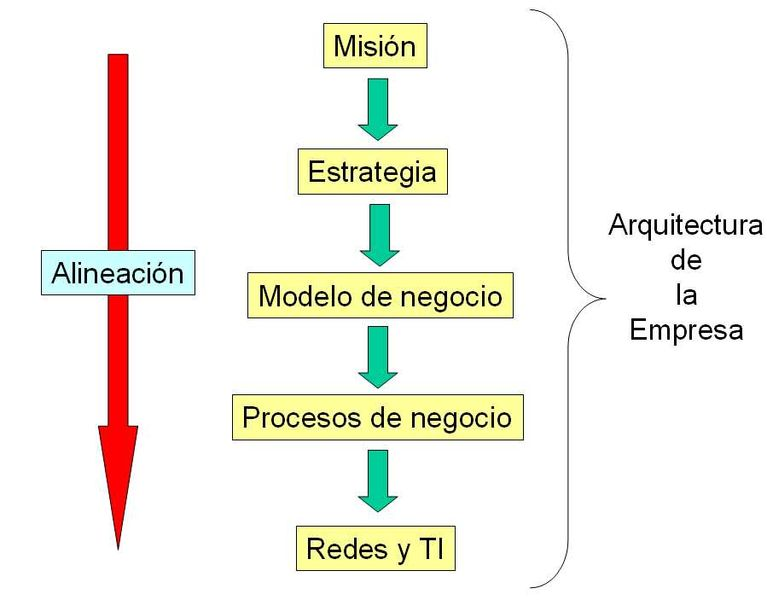
\includegraphics[height=8cm]{images/arqEmpresa}
\end{center}

\begin{itemize}
	\item \emph{Misión:}
		Este es el nivel más alto y explica por qué existe la empresa.
	\item \emph{Estrategia:}
		En este nivel se define qué es lo que se tiene que hacer para cumplir con la misión de la empresa. Se revisa la empresa
		y su entorno externo (es frecuente utilizar técnicas como el análisis SWOT) para decidir cual es el mejor camino para
		maximizar las ganancias dados sus recursos actuales y la posición de la competencia. Es importante tener una visión de
		largo plazo para no caer en la trampa de ganancias a corto plazo que comprometan el futuro de la compañía. Los modelos
		clásicos de competencia son los de Michael Porter: Diferenciación o Liderazgo en costos.
	\item \emph{Modelo de negocio:}
		Este nivel actúa como etapa de conexión entre el nivel Estratégico y el de Procesos de negocio (sin este nivel, la transición
		entre uno y otro es más difícil debido a la ambigüedad que genera el gran paso en el nivel de abstracción). Se explica cómo
		es que la empresa va a generar sus utilidades. Se debe documentar cómo es que las diferentes áreas se relacionan entre sí para
		generar valor para los clientes. Es común describir las etapas de Innovación del producto, Administración de relaciones con los
		clientes, Administración de la Infraestructura, y por último, los Aspectos Financieros (modelo de Yves Pigneur y Alexander
		Osterwalder).
	\item \emph{Procesos de negocio:}
		En este nivel se describen las actividades más importantes de la empresa (el núcleo del negocio). Se sugiere modelar la Cadena
		de valor del negocio y de ahí obtener los procesos del negocio. Los procesos son un conjunto de actividades relacionadas y
		agrupadas que en conjunto reciben un insumo y producen una salida. Dichos procesos pueden automatizarse mediante sistemas de
		cómputo desarrollados a la medida o mediante la compra de sistemas existentes en el mercado como ERP (Planeación de Recursos
		Empresariales) o BPM (Business Process Management)
	\item \emph{Redes y Tecnologías de la Información:}
		Esta etapa se refiere a la tecnología que debe utilizarse para apoyar los procesos de negocio. Claro está que toda la información
		contenida en cualquier tipo de sistema de cómputo no serviría de mucho sin redes de computadoras que permitieran la comunicación
		de dicha información entre clientes, proveedores y la empresa misma.
\end{itemize}
\newpage


\section*{Lo que dice Porter acerca de los procesos de negocios}
\label{sec:procesos}
\subsection*{Definición de proceso}

Un proceso se define como un conjunto de tareas, actividades o acciones interrelacionadas entre sí que,
a partir de una o varias entradas de información, materiales o de salidas de otros procesos, dan lugar
a una o varias salidas también de materiales (productos) o información con un valor añadido.

Hay tres elementos importantes en un proceso:
\begin{itemize}
	\item Valor agregado: Aquellas que transforman los datos e insumos para crear información y productos o servicios para el cliente.
	\item Traspaso (flujo): Aquellas en las que se entrega de manera interdepartamental o externa la información y productos.
	\item Control: Aquellas que permiten que las actividades de traspaso se lleven a cabo de acuerdo a especificaciones previas de calidad, tiempo y costo establecido.
\end{itemize}
Algunos ejemplos de procesos pueden ser los de producción de bienes, entrega de productos o servicios,
el de gestión de las relaciones con los clientes (habitualmente gestionada por un sistema CRM), el de
desarrollo de la estrategia general de la empresa, el de I+D+I de nuevos productos o servicios, etc.

Estos procesos deben estar correctamente gestionados empleando distintas herramientas de gestión de
procesos (en definitiva gestión de la organización) como puede ser un sistema de planificación de
recursos empresariales (ERP), un sistema de Workflow y otros más.

\subsection*{Procesos de negocio}

Un proceso de negocio es un conjunto de tareas relacionadas lógicamente llevadas a cabo para lograr un
resultado de negocio definido. Cada proceso de negocio tiene sus entradas, funciones y salidas. Las
entradas son requisitos que deben tenerse antes de que una función pueda ser aplicada. Cuando una función
es aplicada a las entradas de un método, tendremos ciertas salidas resultantes.

Es una colección de actividades estructurales relacionadas que producen un valor para la organización,
sus inversores o sus clientes. Es, por ejemplo, el proceso a través del que una organización ofrece sus
servicios a sus clientes.

Un proceso de negocio puede ser parte de un proceso mayor que lo abarque o bien puede incluir otros
procesos de negocio que deban ser incluidos en su función. En este contexto un proceso de negocio
puede ser visto a varios niveles de granularidad. El enlace entre procesos de negocio y generación
de valor lleva a algunos practicantes a ver los procesos de negocio como los flujos de trabajo que
efectúan las tareas de una organización. Los procesos poseen las siguientes características:
\begin{enumerate}
	\item Pueden ser medidos y están orientados al rendimiento
	\item Tienen resultados específicos
	\item Entregan resultados a clientes o “stakeholders”
	\item Responden a alguna acción o evento específico
\end{enumerate}
Los procesos de negocio pueden ser vistos como un recetario para hacer funcionar un negocio y alcanzar
las metas definidas en la estrategia de negocio de la empresa.

Hay tres tipos de procesos de negocio:
\begin{enumerate}
	\item Procesos estratégicos - Estos procesos dan orientación al negocio. Por ejemplo, "Planificar estrategia", "Establecer objetivos y metas".
	\item Procesos centrales – Estos procesos dan el valor al cliente, son la parte principal del negocio. Por ejemplo, “Repartir mercancías”
	\item Procesos de soporte – Estos procesos dan soporte a los procesos centrales. Por ejemplo, “contabilidad”, “Servicio técnico”.
\end{enumerate}
Los procesos de negocio consisten en subprocesos, decisiones y actividades.

Un subproceso es parte un proceso de mayor nivel que tiene su propia meta, propietario, entradas y salidas.

Las actividades son partes de los procesos de negocio que no incluyen ninguna toma de decisión ni vale
la pena descomponer (aunque ello sea posible). Por ejemplo, “Responde al teléfono”, “Haz una factura”.

Un proceso de negocio es usualmente el resultado de una Reingeniería de Procesos. El modelado de procesos
es usado para capturar, documentar y rediseñar procesos de negocio.

Vamos a decir que en la época de Taylor un operario realizaba una tarea especifica, y luego se cambió esa
perspectiva en torno a los procesos que son realizados por un trabajo en equipo teniendo en cuenta al cliente
el cual fija las ritmos de los resultados.

Esto facilita el acercamiento y el acuerdo con los clientes, mejora la motivación de los empleados y existe
una mayor facilidad para responder a cambios en el contexto.

Para aplicar los procesos se deben tener claras las tareas, una estructura jerárquica y una tendencia a la
interacción y comunicación vertical.

\subsection*{Metodología esquemática de Reingeniería de Procesos}

Como extremo ideal, se puede establecer una metodología de "papel en blanco", en la que se reinventa toda la
estructura y funcionamiento del proceso o de la organización. Se mantienen los objetivos y estrategias básicas
del negocio, pero se adopta una libertad total de ideas. Esta metodología se puede restringir aprovechando en
mayor o menor medida los procesos ya existentes, haciéndose así un rediseño parcial del proceso.

En cualquiera de los casos, la reingeniería de procesos crea cambios directos y radicales que requieren unas
circunstancias en la organización para adoptarse con éxito:
\begin{itemize}
	\item Sensibilización al cambio.
	\item Planeación estratégica.
	\item Automatización.
	\item Gestión de Calidad Total.
	\item Reestructuración Organizacional.
	\item Mejora Continua.
	\item Valores compartidos.
	\item Perspectiva individual.
	\item Comportamiento en el lugar de trabajo.
	\item Resultados finales.
\end{itemize}
Las etapas de la reingeniería pueden ser las siguientes:
\begin{itemize}
	\item Identificación de los procesos estratégicos y operativos existentes o necesarios, y creación de un mapa (un modelo) de dichos procesos.
	\item Jerarquización del mapa de procesos para su rediseño, y determinación de los procesos clave, aquellos que se abordarán primero o con mayor interés.
	\item Desarrollo de la visión de los nuevos procesos mejorados.
	\item Reingeniería (creación y rediseño) de procesos, realizada por consultores externos, especialistas internos, o una mezcla de ambos.
	\item Preparación y prueba de los nuevos procesos (procesos pilotos).
	\item Procesos posteriores de mejora continúa.
\end{itemize}

\subsection*{La cadena de Valor}

La cadena de valor fue descrita y popularizada por Michael E. Porter en su best-seller de 1985: Competitive Advantage: Creating and Sustaining Superior Performance. New York, NY The Free Press.
Algunas ideas importantes sobre la Cadena de Valor:
\begin{itemize}
	\item Disgrega actividades importantes de la empresa.
	\item La cadena de valor comprende desde el proveedor hasta el cliente.
	\item El obtener y mantener ventajas competitivas depende de comprender y manejar la cadena de valor.
	\item La cadena de valor en las empresas difiere de la empresa, el sector, historia, su estrategia, etc.
\end{itemize}
Tenemos que tener claro que cada empresa es un conjunto de actividades que lleva a cabo para:
\begin{itemize}
	\item Diseñar
	\item Producir
	\item Llevar al mercado
	\item Entregar
	\item Apoyar sus productos
\end{itemize}

Cada actividad de valor emplea insumos, recursos humanos, algún tipo de tecnología para desempeñar su función.
Cada actividad de valor utiliza y crea información. (por ejemplo: datos del comprador, parámetros de desempeño de maquinaria, estadísticas de fallas del producto, etc.).

La Cadena de Valor categoriza las actividades que producen valor añadido en una organización. Se dividen en dos tipos de actividades:
\begin{itemize}
	\item Las actividades primarias que conforman la creación física del producto, las actividades relacionadas con su venta y la asistencia post-venta. Se dividen en:
	\begin{itemize}
		\item Logística interna: recepción, almacenamiento y distribución de las materias primas.
		\item Operaciones (producción): recepción de las materias primas para transformarlas en el producto final.
		\item Logística externa: almacenamiento de los productos terminados y distribución del producto al consumidor.
		\item Ventas y Marketing: actividades con las cuales se da a conocer el producto.
		\item Servicios post-venta (mantenimiento): actividades destinadas a mantener o realizar el valor del producto. Ej: garantías
	\end{itemize}
	\item Estas actividades son apoyadas por las también denominadas actividades secundarias:
	\begin{itemize}
		\item Infraestructura de la organización: actividades que prestan apoyo a toda la empresa, como la planificación, contabilidad, finanzas...
		\item Dirección de recursos humanos: búsqueda, contratación y motivación del personal.
		\item Desarrollo de tecnología (investigación y desarrollo): obtención, mejora y gestión de la tecnología.
		\item Abastecimiento (compras): proceso de compra de los materiales.
	\end{itemize}
\begin{center}
	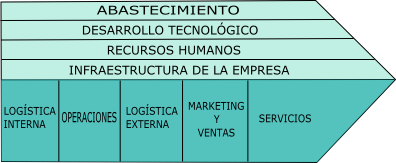
\includegraphics[height=4cm]{images/cadenaDeValor}
\end{center}

\end{itemize}

\subsubsection*{Tipos de Actividad}
Dentro de cada categoría de actividades primarias y de apoyo, hay tres tipos de actividades que juegan un papel diferente en la ventaja competitiva:
\begin{itemize}
	\item Directas: Actividades implicadas directamente en la creación de valor para el comprador: ensamble, maquinado de partes, operación de la fuerza de ventas,etc.
	\item Indirectas: Actividades que hacen posible el desempeñar las actividades directas en una base continua, como mantenimiento, programación, operación de las instalaciones, etc.
	\item Seguro de calidad: Actividades que aseguran la calidad de otras actividades (monitoreo, inspección, pruebas, revisión, etc.)
\end{itemize}
Ademas Para cada actividad de valor añadido han de ser identificados los generadores de costes y valor.

\subsubsection*{El marco de la cadena}

La cadena de valor enseguida se puso en el frente del pensamiento de gestión de empresa como una poderosa
herramienta de análisis para planificación estratégica. Su objetivo último es maximizar la creación de valor
mientras se minimizan los costos. De lo que se trata es de crear valor para el cliente, lo que se traduce
en un margen entre lo que se acepta pagar y los costos incurridos.

La cadena de valor ayuda a determinar las actividades que permiten generar una Ventaja Competitiva (también
expresado por Michael Porter). Tener una ventaja competitiva es tener una rentabilidad relativa superior a
los rivales en el sector industrial en el cual se compite, la cual tiene que ser sustentable en el tiempo.
Rentabilidad significa un margen entre los ingresos y los costos. Cada actividad que realiza la empresa debe
generar el mayor posible. De no ser así, debe costar lo menos posible, con el fin de obtener un margen superior
al de los rivales. Las Actividades de la cadena de valor son múltiples y además complementarias (relacionadas).
El conjunto de actividades de valor que decide realizar una unidad de negocio es a lo que se le llama estrategia
competitiva (también expresado por Porter) o estrategia del negocio (diferente a las estrategias corporativas
o a las estrategias de un área funcional).

El concepto ha sido extendido más allá de las organizaciones individuales. También puede ser aplicado a cadenas
de suministro completas así como a redes de distribución. La puesta a disposición de un conjunto de productos y
servicios al consumidor final moviliza diferentes actores económicos, cada uno de los cuales gestiona su cadena
de valor. Las interacciones sincronizadas de esas cadenas de valor locales crean una cadena de valor ampliada que
puede llegar a ser global. Capturar el valor generado a lo largo de la cadena es la nueva aproximación que han
adoptado muchos estrategas de la gestión. A base de explotar la información que se dirige hacia arriba y hacia
abajo dentro de la cadena, las compañías pueden intentar superar los intermediarios creando nuevos modelos de negocio.

\subsubsection*{Valor Agregado vs Cadena de Valor}
Valor agregado es el precio de venta menos el costo de la materia prima comprada.
El valor agregado no es una base sólida de análisis de costos y ventajas competitivas ya que no distingue el costo de materias primas.
De muchos otros insumos que son adquiridos (comprados) que se utilizan en las actividades de una empresa.
El comportamiento de los costos no puede ser comprendido sin examinar simultáneamente los costos de los insumos usados para lograrlos.
En la Cadena de Valor realza las relaciones entre la empresa y sus proveedores, lo que puede reducir el costo o aumentar la diferenciación.
(la diferencia que una empresa establece al proporcionar algo único que es valioso para los compradores más allá de ofrecer un precio bajo).

\subsubsection*{Eslabones dentro de la Cadena de Valor}
La Cadena de Valor es un sistema de actividades interdependientes relacionadas por eslabones o relaciones entre la manera en que se desempeñe una actividad y el costo o desempeño de otra.
Los eslabones pueden llevar a la ventaja competitiva de dos maneras:
\begin{itemize}
	\item Optimización
	\item Coordinación
\end{itemize}
Los eslabones surgen de:
\begin{itemize}
	\item La misma función puede ser desempeñada de diferentes formas.
	\item El costo de desempeño de las actividades directas se puede mejorar por mayores esfuerzos de actividades indirectas.
	\item Actividades desempeñadas dentro de una empresa reducen la necesidad de mostrar, explicar o dar servicio a un producto en el campo.
	\item Las funciones de seguro de calidad pueden ser desempeñadas de diferentes maneras.
\end{itemize}
Los eslabones son cruciales en la Cadena de Valor pero muchas veces son sutiles y pasan desapercibidos.
La identificación de los eslabones es un proceso de búsqueda de maneras en que las que cada actividad de valor afecta o es afectada por otras.

\subsubsection*{Eslabones Verticales}
Los eslabones no sólo existen dentro de la Cadena de Valor de la empresa, sino entre la cadena de una empresa y las Cadenad de Valor de los proveedores y los canales.
También hay cadena de valor de comprador y la forma en que se relaciona con la Cadena de Valor de la empresa, marca diferenciación.

La Cadena de Valor despliega el valor total y consiste de las actividades de valor y del margen.
El margen es la diferencia entre el valor total y el costo colectivo de desempeñar las actividades de valor.

\newpage


%fin desarrollo

\section*{Conclusiones}
\label{sec:conclusiones}
%De acuerdo a la introducci\'on que se hizo, entregar afirmaciones
%  basadas en los experimientos y sus resultados.

A primera vista, los resultados obtenidos en la presente implementación, superan en gran medida a los óptimos encontrados
en todos estos años, donde distintas personas, han utilizado, variadas técnicas para poder resolver el \emph{Car Sequencing Problem}
de la mejor manera, considerando así, que se pudieron haber utilizado técnicas completas, que si bien es cierto, pueden demorar mucho,
van a encontrar el \emph{óptimo global} de un determinado problema, lo cual se diferencia notoriamente con las técnicas incompletas,
como es el caso de ka presente implementación, donde sólo se puede encontrar un \emph{óptimo local}.

Al mirar el gráfico podemos darnos cuenta, de que la distribución de la cantidad de restricciones violadas, poseen un comportamiento
bastante similar, guardando las proporciones de la cantidad de violaciones, lo que nos hace deducir, de que sólo nos falta un poco
más de control y sintonización de los parámetros utilizados, para acercarnos aún más a soluciones más óptimas.

Siguiendo con el análisis de los experimentos, podemos darnos cuenta de que si bien es cierto, las soluciones violan una cantidad
considerable de restricciones, estamos sacrificando una buena solución, por un corto tiempo de ejecución, el cual en algunos casos,
sólo llega a durar 1 minuto, lo que comparado con el tiempo de alguna técnica completa, que puede durar días, nos beneficia de cierta manera.

Con respecto a la representación del problema, existen ciertos pros y contras.
Primero que todo la representación que se utilizó en la presente implementación,
consiste en una del tipo no-binaría, por lo que no es tan fácil utilizar los típicos movimientos de las representaciones binarias,
como lo son el \emph{bit-flip} y el \emph{cruzamiento en un punto}, ya que estaríamos violando las restricciones duras del problema,
por lo cual en la presente implementación, por ejemplo, no se utilizó un operador de cruzamiento y sólo se deposito la confianza,
en la mutación con \emph{Simulated Annealing} que se encargó tanto de explorar como de explotar.

Según lo anteriormente dicho, el no poseer un operador de cruzamiento, puede haber perjudicado la explotación del presente algoritmo
evolutivo, y por ende, entorpecido la búsqueda de un óptimo local. Aunque los resultados no fueron del todo malos, por lo que el simulated annealing
hizo su trabajo explorando y explotando, pero no de la forma más apropiada.

Otro punto importante en la presente implementación, es la forma en la cual se genera la población inicial.
Como ya hemos mencionado anteriormente, lo favorable del método utilizado es que se generan soluciones factibles,
es decir, que cumplen las restricciones duras, pero por otro lado, éstas se generan de forma aleatoria, lo cual indica,
que quizás utilizando alguna técnica de construcción de individuos más apropiada, como Greedy o GRASP, la calidad de la
población inicial aumentaría, lo cual sería interesante como trabajo futuro.


Con respecto a la mutación con simulated annealing, cabe señalar que existen algunos aspectos que pueden ser mejorados,
como por ejemplo un control de la temperatura, pues en la presente implementación, la temperatura disminuye cada 3 iteraciones,
lo que si tomamos en cuenta un control más riguroso, como comparar la calidad de las soluciones generadas, podríamos
realizar los cambios en la temperatura, a medida que el algoritmo se comporta de una forma más apropiada.


Finalmente, es posible mejorar la presente implementación de un algoritmo evolutivo aumentando la exploración,
que en éste caso significa poder mejorar lo que es la mutación, ya que dentro del simulated annealing, el movimiento
no es muy apropiado, y quizás el sólo hecho de mejorar el movimiento de la mutación simulated annealing, puede
traer un mejor desempeño en nuestro algoritmo. Otra forma podría ser cambiar el método de la ruleta, pues si bien es cierto,
le entrega una mayor probabilidad para escoger los mejores individuos, no nos prohibe elegir malos individuos, lo que
perjudica a nuestra siguiente población, y por ende a la solución del problema.


% OLD

%Conclusiones revelantes del estudio realizado.

%En el presente informe se ha dado un estado del arte de un problema muy popular
%en el área de la inteligencia artificial, el \emph{Car Sequencing Problem}, siendo éste
%una variación de otro problema connotado llamado \emph{Job Shop Scheduling}.
%Es tanto la importancia del presente problema, que la \emph{French Society of Operations
%Research and Decision-Making Aid} ha decidido ya hace varios años, comenzar lo que se denomina
%\emph{The ROADEF challenge} cada dos años, teniendo como objetivo central,  permitir a las personas
%que se desarrollan en el área de la industria el presenciar todos los avances y evoluciones
%en el ámbito de la Investigación de Operaciones y Análisis de Decisiones, pero no sólo eso
%sino el poder enfrentar directamente problemas decisionales complejos, que ocurren en la industria.
%Siguiendo la idea anterior, lo importante de éste \emph{Challenge} es que en el 2005, se consideró
%como tema principal el \emph{Car Sequencing Problem} debido a la propuesta que realizó RENAULT,
%por lo cual uno podrá imaginar la cantidad de avances que se produjeron, pues cada participante
%abordaba el problema desde una metodología distinta.
%
%Por otra parte, pareciera que un problema relacionado a \emph{ordenar} un conjunto de vehículos
%para ser ensamblados y así obtener el orden más óptimo, no es una tarea difícil, pero claramente
%debido a la complejidad que otorgan las restricciones y de que es un problema de la vida real,
%presenta un grado de dificultad mayor, lo cual queda reflejado por la cantidad de publicaciones 
%e investigaciones que hay al respecto.
%
%Se dieron a conocer también, tres áreas para atacar el presente problema.
%Por un lado tenemos los métodos heurísticos que como bien sabemos, es prácticamente jugar a la ruleta
%rusa con nuestra investigación, pues la heurística solamente selecciona un objetivo de los dos provenientes
%de la definición, una buena solución o un buen tiempo de ejecución. Pero también se presenta que la heurística
%es un mecanismo confiable para decidir \emph{utilizarlo} como un apoyo, mas que utilizarlo solo.
%
%Siguiendo con los mecanismos planteados, se vieron también los  métodos exactos,
%es decir, técnicas de optimización, donde podemos encontrar la \emph{programación lineal entera},
%\emph{branch and bound} y \emph{local search}, los cuales se dedicaban netamente a construir una
%solución óptima a partir de los datos que el mismo problema nos entrega. El único problema que tienen
%éstas técnicas es que la complejidad temporal va a crecer demasiado con respecto al tamaño de nuestro
%\emph{input} del algoritmo.
%
%Dentro de toda la lectura realizada para las distintas técnicas, pude percatarme que las mejores soluciones
%siempre son variaciones de métodos o tomar dos técnicas como complementarias, por ejemplo uno de los
%mejores resultados fue la combinación de un \emph{Ant Colony Optimization} con una heurística dinámica,
%pues claramente se nos señala que el buen uso de una heurística es crucial, es decir, hay que preocuparse
%de leer los estudios que se han publicado, par ver cual es la combinación más óptima.
%
%Finalmente, es impresionante la cantidad de estudios con respecto a éste problema en particular,
%por lo que podemos darnos cuenta que muchos centros de investigación han dedicado tiempo valioso
%para la resolución óptima del \emph{Car Sequencing Problem}, pero no tanto la versión que se estudió,
%que es la propuesta por Parello~\cite{parello}, sino mas bien al desafío de la ROADEF.


\section*{Referencias}
\label{sec:referencias}
\begin{itemize}
	\item http://drfd.hbs.edu/fit/public/facultyInfo.do?facInfo=bio\&facEmId=mporter
	\item http://es.wikipedia.org/wiki/Michael\_Porter
	\item http://es.wikipedia.org/wiki/Cadena\_de\_valor
	\item http://es.wikipedia.org/wiki/Reingeniería\_de\_Procesos
	\item http://www.12manage.com/methods\_porter\_value\_chain\_es.html
\end{itemize}
\newpage


\section*{Glosario}
\label{sec:glosario}
\begin{itemize}
	\item \emph{Actividades generadoras de valor:} Suma de los beneficios percibidos
		 por un cliente menos los costos en los que incurre por adquirir y usar el
		 producto o servicio (definición según Porter).
	\item \emph{Actividades de valor:}  Son las distintas actividades que puede desarrollar
		 la empresa, por margen entendemos la diferencia entre el valor total y el costo
		 colectivo de desempeñar las actividades de valor.
	\item \emph{Cadenas de valor:} Son una forma de análisis de la actividad empresarial, que
		 se basa en descomponer las funciones constitutivas, en actividades generadoras
		 de valor, buscando identificar fuentes de ventaja competitiva, ya sea reduciendo
		 costos u optando por la diferenciación.
	\item \emph{Empresa:} Es la actividad donde involucro la planeación, organización, dirección
		 y control de recursos de mano de obra, de producción, finanzas, ventas, etc, enfocando
		 los esfuerzos, en la mayoría de los casos a la obtención de lucro.
	\item \emph{Estrategía:} Es la teoría que la alta dirección tiene sobre la base para sus éxitos
		 pasados y futuros. Es una herramienta de dirección que facilita procedimientos y
		 técnicas con un basamento científico, que empleadas de manera iterativa y transfuncional,
		 contribuyen a lograr una interacción proactiva de la organización con su entorno,
		 coadyuvando a lograr efectividad en la satisfacción de las necesidades del público
		 objetivo a quien está dirigida la actividad de la misma.
	\item \emph{Gestión de la información:} Su valorización permite entender las organizaciones como
		 sistemas de interpretación y acción que incrementan el potencial competitivo, siempre
		 bajo un doble prisma individual y colectivo. es quien gestiona la compra y la carga de
		 los documentos y acaba convirtiéndose en un controlador de acceso a las informaciones
	\item \emph{Margen:} Diferencia entre el valor total y el costo colectivo de desempeñar las
		 actividades de valor.
	\item \emph{Mercadotecnia:} Actualmente representa una herramienta fundamental en la recopilación
		 y análisis de la información, para transformarla en elemento clave en la toma de decisiones,
		 que llevará sus productos o servicios con éxito hasta sus consumidores.
	\item \emph{SI (Sistema de Información):} Conjunto de componentes interrelacionados que permiten
		 capturar, procesar, almacenar y distribuir la información para apoyar la toma de decisiones
		 y el control en una institución.
	\item \emph{TI (Tecnologías de la Información):} Herramienta esencial para gestionar la productividad

	\item \emph{Ventajas competitivas:} Se logra cuando la empresa desarrolla e integra las actividades
		 de su cadena de valor de forma menos costosa y mejor diferenciada que sus rivales. 
	\item \emph{RP:} Comprendiendo qué es un proceso y cómo este forma parte integral de las empresas e
		 instituciones, cuales quiera sea su naturaleza, es posible entonces llegar a una definición.
		 Hammer y Champy definen a la RP como “la reconcepción fundamental y el rediseño radical de los
		 procesos de negocios para lograr mejoras dramáticas en medidas de desempeño tales como en costos,
		 calidad, servicio y rapidez” (Fuente: Institute of Industrial Engineers, "Más allá de la
		 Reingeniería", CECSA, México, 1995, p.4). Por lo tanto se trata de una reconcepción fundamental
		 y una visión holística de una organización. Preguntas como: ¿por qué hacemos lo que hacemos? y
		 ¿por qué lo hacemos como lo hacemos?, llevan a interiorizarse en los fundamentos de los procesos
		 de trabajo. La RP es radical hasta cierto punto, ya que busca llegar a la raíz de las cosas,
		 no se trata solamente de mejorar los procesos, sino y principalmente, busca reinventarlos.
	\item \emph{Costo:} Es la valorización monetaria de la suma de recursos y esfuerzos que han de invertirse
		 para la producción de un bien o de un servicio. El precio y gastos que tienen una cosa, sin
		 considerar ninguna ganancia.
	\item \emph{Valor:} Es la cantidad de dinero que los clientes están dispuestos a pagar por los productos o
		 servicios de la empresa.
	\item \emph{Empresa:} Es la unidad productora de bienes y servicios homogéneos para lo cual organiza y
		 combina el uso de factores de la producción.
	\item \emph{Capital:} Es el total de recursos fíisicos y financieros que posee un ente económico, obtenidos
		 mediante aportaciones de los socios o accionistas destinados a producir beneficios, utilidades
		 o ganancias.
	\item \emph{Producto:} Es el punto central de la oferta que realiza toda empresa u organización (ya sea
		 lucrativa o no) a su mercado meta para satisfacer sus necesidades y deseos, con la finalidad
		 de lograr los objetivos que persigue.
	\item \emph{Outsourcing:} Es el proceso en el cual una firma identifica una porción de su proceso de ne-
		 gocio que podrá ser desempeñada más eficientemente y/o más efectivamente por otra
		 corporación, la cual es contratada para desarrollar esa porción de negocio.

\end{itemize}
\newpage


\section*{M\'etodo de Trabajo}
\label{sec:metodo}
Bueno aunque siempre se describe el método de trabajo grupal en este caso
ésta tarea se realizaba de manera individual, de todas formas el mecanismo
para poder realizar el informe fue el siguiente.

Lei el texto de cadena de valor, trate de entender sus ideas principales para
poder tener una idea general de lo que se trata el texto. Por otro lado comence
a buscar otros informes en internet que tuvieran relacion con Porter y la cadena
de valor y los procesos de negocios, para poder tener el suficiente material
para poder presentar un informe.



\newpage


\end{document}
